% Created 2024-10-18 Fri 17:38
% Intended LaTeX compiler: pdflatex
\documentclass[11pt]{article}
\usepackage[utf8]{inputenc}
\usepackage[T1]{fontenc}
\usepackage{graphicx}
\usepackage{longtable}
\usepackage{wrapfig}
\usepackage{rotating}
\usepackage[normalem]{ulem}
\usepackage{amsmath}
\usepackage{amssymb}
\usepackage{capt-of}
\usepackage{hyperref}
\usepackage{parskip,darkmode}
\enabledarkmode
\usepackage{tikz}
\author{Arnav Gupta}
\date{\today}
\title{Supervised Machine Learning: Foundations}
\hypersetup{
 pdfauthor={Arnav Gupta},
 pdftitle={Supervised Machine Learning: Foundations},
 pdfkeywords={},
 pdfsubject={},
 pdfcreator={Emacs 29.4 (Org mode 9.7.11)}, 
 pdflang={English}}
\begin{document}

\maketitle
\tableofcontents

\section{Learning}
\label{sec:org24e290b}
The ability to improve behaviour based on experience.
Improvements can be:
\begin{itemize}
\item \textbf{range} of behaviours is expanded: agent can do more
\item \textbf{accuracy} on tasks is improved: agent can do things better
\item \textbf{speed} is improved: agent can do things faster
\end{itemize}

Components of a learning problem:
\begin{itemize}
\item \textbf{task}: behaviour being improved
\item \textbf{data}: experiences used to improve performance in the task
\item \textbf{measure of improvement}
\end{itemize}

Common learning tasks include:
\begin{itemize}
\item \textbf{supervised classification}: given a set of pre-classified data, classify a new instance
\item \textbf{unsupervised learning}: find natural classes for examples
\item \textbf{reinforcement learning}: determine what to do based on rewards and punishments
\item \textbf{transfer learning}: learn from an expert
\item \textbf{active learning}: learner actively seeks to learn
\item \textbf{inductive logic programming}: build richer models in terms of logic programs
\end{itemize}

Learning tasks can be characterized by the feedback given to the learner:
\begin{itemize}
\item for supervised learning, what has to be learned is specified per example
\item for unsupervised learning, no classifications given so learner must discover categories and regularities
in data
\item for reinforcement learning, feedback occurs after a sequence of actions
\end{itemize}
\subsection{P/N Agents}
\label{sec:org8da326e}
Measure of success is how well the agent performs on new, unseen examples.

For two agents solving a binary classification task:
\begin{itemize}
\item \(P\) claims the negative examples seen are the only negative examples (all others positive)
\item \(N\) claims the positive examples seen are the only positive examples (all others negative)
\end{itemize}

Both agents correctly classify every training example, but disagree on every other example.
They use training data as their model, needing an exact match.
\subsubsection{Bias}
\label{sec:org93cbd1a}
Tendency to prefer one hypothesis over another.
Necessary to make predictions on unseen data.

To make predictions on unseen data, bias is necessary.
Good biases must be tested to find out their quality.
\subsection{Learning as Search}
\label{sec:org101ea58}
Given a representation and bias, learning is search through all possible representations looking
for the representation(s) that best fit the data, given the bias.

Learning algorithm is made of:
\begin{itemize}
\item search space (possible representations)
\item evaluation function
\item search method
\end{itemize}
\section{Supervised Learning}
\label{sec:org7c88203}
Supervised learning requires:
\begin{itemize}
\item a set of input features \(X_{1}, \dots, X_{n}\)
\item a set of target features \(Y_{1}, \dots, Y_{k}\)
\item a set of training examples with values given for input features and target features
\item a set of test examples where only values for input features are given
\end{itemize}

\uline{Goal}: Predict values of target features for test examples using
\begin{itemize}
\item classification when target features are discrete
\item regression when target features are continuous
\end{itemize}
\subsection{Noise}
\label{sec:org4fab7a9}
Data can have:
\begin{itemize}
\item some features assigned the wrong value
\item inadequate features to predict classification
\item missing features
\end{itemize}

\textbf{Overfitting}: distinction appears in training data but not in test data, due to random correlations
\section{Measures of Error}
\label{sec:org6f981b4}
For a feature \(Y\) and example \(e\):
\begin{itemize}
\item \(Y(e)\) is the value of feature \(Y\) for \(e\)
\item \(\hat{Y}(e)\) is the predicted value of feature \(Y\) for \(e\)
\item \textbf{error} of prediction: measure of how how close \(Y(e)\) and \(\hat{Y}(e)\) are
\end{itemize}

Let \(E\) be a set of examples and \(T\) be a set of target features:
\begin{itemize}
\item \textbf{absolute error}
$$
  \sum_{e \in E} \sum_{Y \in T} \left| Y(e) - \hat{Y}(e) \right|
  $$
\item \textbf{sum of squares error}
$$
  \sum_{e \in E} \sum_{Y \in T} \left( Y(e) - \hat{Y}(e) \right)^{2}
  $$
\item \textbf{worst case error}
$$
  \max_{e \in E} \max_{Y \in T} \left| Y(e) - \hat{Y}(e) \right|
  $$
\item \textbf{cost-based error}: takes into account costs of various errors
\end{itemize}

For the case where target features are \(Y(e) \in \{0, 1\}\) and predicted features are
\(\hat{Y}(e) \in [0, 1]\):
\begin{itemize}
\item \textbf{likelihood of the data}:
$$
  \prod_{e \in E} \prod_{Y \in T} P(\hat{Y}(e) \mid Y(e))
  $$
$$
  \prod_{e \in E} \prod_{Y \in  T} \hat{Y}(e)^{Y(e)} (1 - \hat{Y}(e))^{(1 - Y(e))}
  $$
\item \textbf{entropy} or \textbf{negative log likelihood}
$$
  -\sum_{e \in E} \sum_{Y \in T} \left[ Y(e) \log( \hat{Y}(e) ) + (1 - Y(e)) \log ( 1 - \hat{Y}(e) ) \right]
  $$
\end{itemize}
\subsection{Precision and Recall}
\label{sec:orgdbb25f3}
\textbf{Recall} or \textbf{sensitivity}
$$
\frac{\text{true positives}}{\text{true positives} + \text{false negatives}}
$$

\textbf{Specificity}
$$
\frac{\text{true negatives}}{\text{true negatives} + \text{false positives}}
$$

\textbf{Precision}
$$
\frac{\text{true positives}}{\text{true positives} + \text{false positives}}
$$

\textbf{F1-measure}
$$
\frac{2 \times \text{Precision} \times \text{Recall}}{\text{Precision} + \text{Recall}}
$$

The \textbf{receiver operating curve} gives the full range of performance of an algorithm across different
biases.

\begin{center}
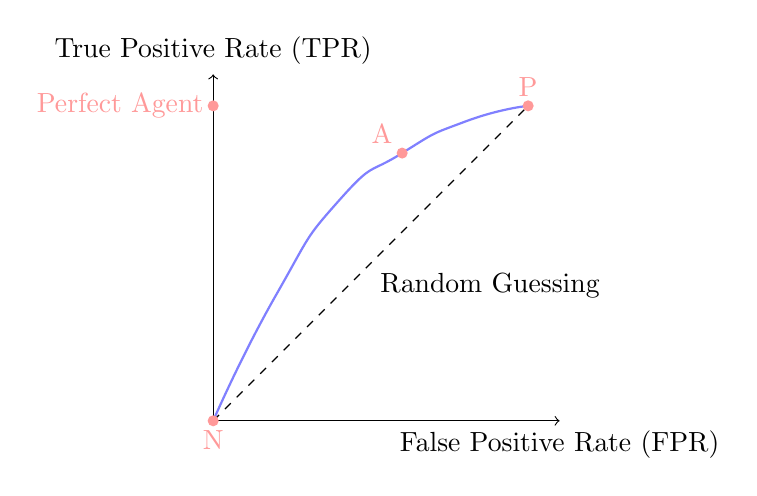
\begin{tikzpicture}[scale=4]
    % Axes
    \draw[->] (0,0) -- (1.1,0) node[below] {False Positive Rate (FPR)};
    \draw[->] (0,0) -- (0,1.1) node[above] {True Positive Rate (TPR)};

    % Curved ROC curve
    \draw[thick, blue!50] plot [smooth, tension=1] coordinates {(0,0) (0.2,0.4) (0.4,0.7) (0.6,0.85) (0.8,0.95) (1,1)};

    % Diagonal line
    \draw[dashed] (0,0) -- (1,1) node[pos=0.5, below right] {Random Guessing};

    % Points on the curve
    \fill[red!40] (0,0) circle (0.5pt) node[below] {N};
    \fill[red!40] (0,1) circle (0.5pt) node[left] {Perfect Agent};
    \fill[red!40] (0.6,0.85) circle (0.5pt) node[above left] {A};
    \fill[red!40] (1,1) circle (0.5pt) node[above] {P};

\end{tikzpicture}
\end{center}
\end{document}
